%%%%%%%%%%%%%%%%%%%%%%%%%%%%%%%%%%%%%%%%%%%%%%%%%%%%%%%%%%%%%%%%%%%%%%%%%%%%%%%%%%%%%%%%%%

%%%%%%%%%%%%%%%%%%%%%%%%%%%%%%%%%%% Author:Yao Zhang  %%%%%%%%%%%%%%%%%%%%%%%%%%%%%%%%%%%%
%%%%%%%%%%%%%%%%%%%%%%%%%%%%% Email: jaafar_zhang@163.com  %%%%%%%%%%%%%%%%%%%%%%%%%%%%%%%

%%%%%%%%%%%%%%%%%%%%%%%%%%%%%%%%%%%%%%%%%%%%%%%%%%%%%%%%%%%%%%%%%%%%%%%%%%%%%%%%%%%%%%%%%%

\documentclass[aspectratio=2516]{beamer}
\mode<presentation> {
\usetheme{Madrid}
%\setbeamertemplate{footline} % To remove the footer line in all slides uncomment this line
}

\usepackage{graphicx} 
\graphicspath{ {img/} }
\usepackage[caption=false, font=footnotesize]{subfig}
\setbeamertemplate{caption}[numbered]
\newtheorem{remark}{Remark}
\newtheorem{coro}{Corollary}
\newtheorem{thm}{Theorem}
\newtheorem{eg}{Example}
\newtheorem{proposition}{Proposition}
\newtheorem{lma}{Lemma}
\usepackage{algorithm}
\usepackage{algorithmic}
\renewcommand{\algorithmicrequire}{\textbf{Input:}}  
\renewcommand{\algorithmicensure}{\textbf{Output:}} 
\setbeamertemplate{theorems}[numbered]
\usepackage{bbding}
%\usepackage{ctex}
\renewcommand{\figurename}{Figure}
\renewcommand{\tablename}{Table}

%----------------------------------------------------------------------
\title[Follow Your Heart]{ When You Follow Your Heart} % The short title appears at the bottom of every slide, the full title is only on the title page
\vspace{0.5cm}
\subtitle{ You Cease Having Regrets}
\vspace{2.5cm}


\author{Yao Zhang} % 

\institute[UCAS \& NAOC] 
{	
    
    University of Chinese Academy of Sciences \\
     
	\vspace{0.2cm}
	
	 National Astronomical Observatories, Chinese Academy of Sciences \\
	 
	 \vspace{0.5cm}
	
     {\color{blue} \url{https://zhims.github.io}}
}

\date{\today}


\logo{
\includegraphics[height=0.6cm]{yao.jpg}}

%----------------------------------------------------------------------
\begin{document}
	\begin{frame}
	\titlepage 
	\end{frame}
%-----------------------------------------------------------------------
\begin{frame}
\frametitle{Overview} 
\begin{small}
	\tableofcontents
\end{small} 
\end{frame}

%----------------------------- section 1 -------------------------------------------
\section{Introduction}
%-----------------------------------------------------------------------------------

\begin{frame}
\frametitle{ Section \uppercase\expandafter{\romannumeral1}}


\begin{center}
	\Large Our Academic Family
\end{center}

\end{frame}
%------------------------------------------------------------------------------------

\begin{frame}
\frametitle{Our Academic Family}


\begin{figure}
	\centering
	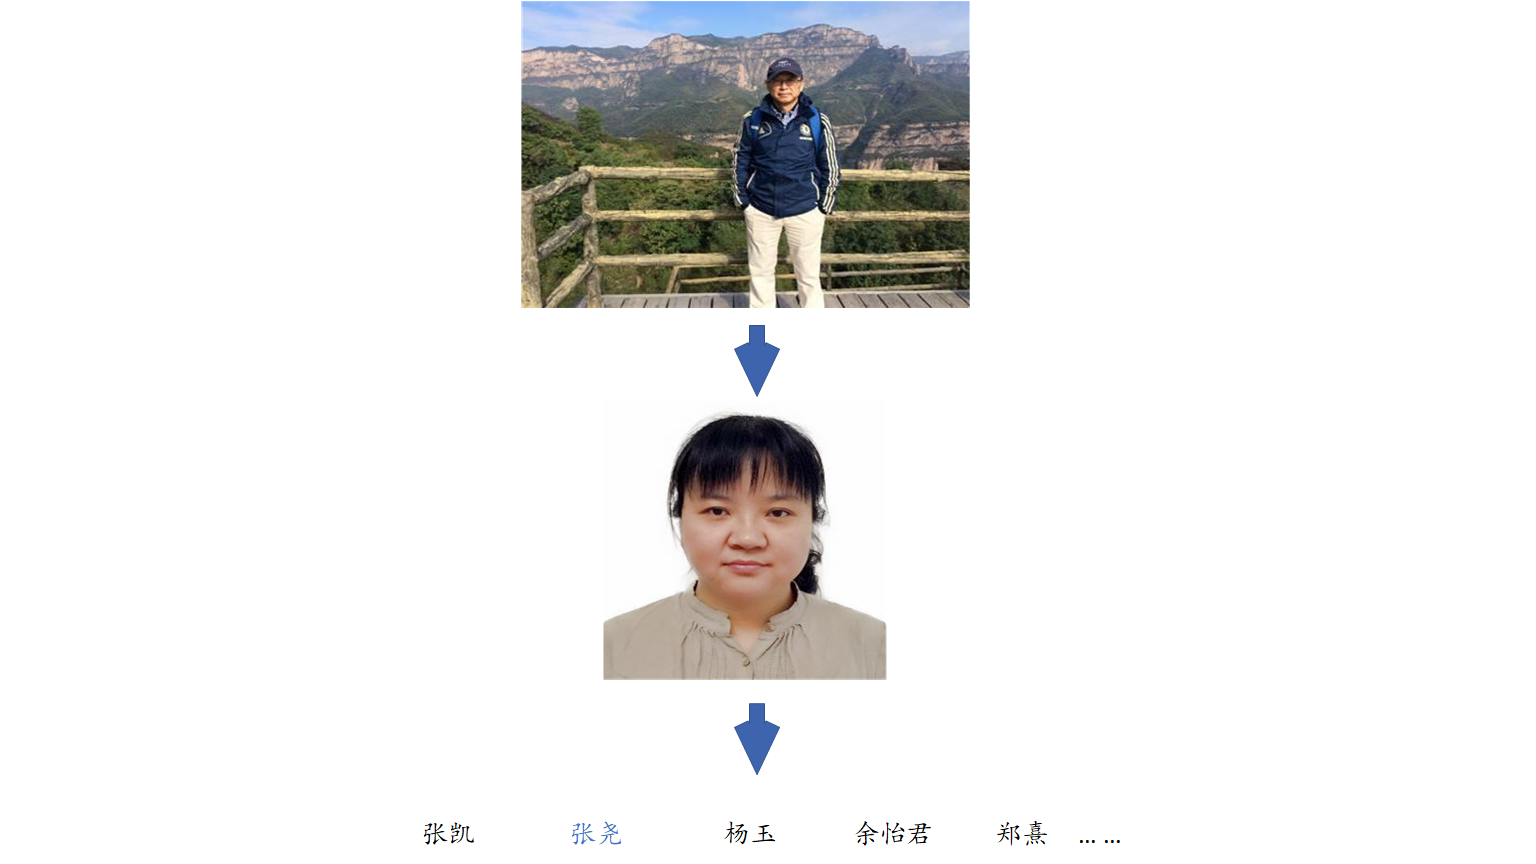
\includegraphics[width=0.9\linewidth,height=0.5\linewidth]{yao_zhang.png}
	\caption{Our Academic Family}
	\label{fig1} 
\end{figure}

\end{frame}



%-----------------------------------------------------------------------------------


\begin{frame}

\frametitle{Introduction}
 
 \begin{center}
 	\color{blue} \Large Computing Science VS Computer Science
 \end{center}

\end{frame}

%-----------------------------------------------------------------------------------
%----------------------------- section 2 -------------------------------------------
\section{Low Rank and Sparse Based on Matrix}
%-----------------------------------------------------------------------------------

\begin{frame}
\frametitle{ Section \uppercase\expandafter{\romannumeral2}}


\begin{center}
	\Large Low Rank and Sparse based on Matrix
\end{center}

\end{frame}

%-----------------------------------------------------------------------------------

\begin{frame}

\frametitle{\small Why Are Big Data Matrices Approximately Low Rank? }

\begin{lma}[Johnson--Lindenstrauss Lemma]
	Given $ 0 < \epsilon < 1 $, as set of $ m  $ points in $ \mathbb{R}^{N} $, and a number $n > 8\frac{{\log \;m}}{{{\varepsilon ^2}}}$, there is a linear map, $f:\;{\mathbb{R}^N} \to {\mathbb{R}^n}$ such that 
	
	\begin{equation}
	\left( {1 - \varepsilon } \right){\left\| {u - v} \right\|^2} \leqslant {\left\| {f\left( u \right) - f\left( v \right)} \right\|^2} \leqslant \left( {1 + \varepsilon } \right){\left\| {u - v} \right\|^2}
	\end{equation}
	
\end{lma}

\vspace{1cm}

There is a recommended paper {\color{blue} \cite{p1}}.

\end{frame}
%-----------------------------------------------------------------------------------

\begin{frame}

\frametitle{\small Why Are Big Data Vectors or Matrices Approximately Sparse Representation? }

Given $ X \in \mathbb{R}^{m\times n} $, 

\begin{equation}
{\left\| X \right\|_*} = {\left\| \Sigma  \right\|_1}
\end{equation}

\vspace{0.5cm}

where $X = U\sum {V^T},\;U{U^T} = {I_{m \times m}},V{V^T} = {I_{n \times n}}$.

\vspace{1cm}

{\tiny  There is an additional slides: {\color{blue} \url{http://stanford.edu/~qysun/Lecture04_SunQY.pdf}} which introduce sparsity in Convolutional Neural Networks}.

\vspace{0.5cm}

\end{frame}

%-----------------------------------------------------------------------------------
\begin{frame}

\frametitle{ Generalized PCA VS Representation Theory}

Generalized PCA model:

\begin{equation}
\begin{split}
\mathop {\min }\limits_{L,S} \;{\left\| L \right\|_{rank}}\; + \;\lambda{\left\| S \right\|_{sparse}} \quad \ s.t. \ X = L + S 
\end{split}
\end{equation}

\vspace{1cm}

Representation theory model:
\begin{equation}
\begin{split}
\mathop {\min }\limits_{D,C,E} \;{\left\| C \right\|_{rank\;or\;sparse}}\; + \;\lambda{\left\| E \right\|_{p - norm}}\;s.t.\;X = DC + E
\end{split}
\end{equation}


\end{frame}
%-----------------------------------------------------------------------------------
%-----------------------------------------------------------------------------------

\begin{frame}
\frametitle{\small One Easy Approach to Solving Low Rank and Sparse Models}

We want to get that:

\begin{equation}
\begin{split}
\small 
\mathop {\min }\limits_X \tau {\left\| X \right\|_*} & + \frac{1}{2}\left\| {X - A} \right\|_F^2\\
\mathop {\min }\limits_X \tau {\left\| X \right\|_1} & + \frac{1}{2}\left\| {X - A} \right\|_F^2
\end{split}
\end{equation}

\vspace{-0.25cm}

\begin{example}
	\begin{enumerate}
		\item \small Robust Principal Component Analysis (RPCA) model:
		\begin{equation}
		\small 
		\mathop {\min }\limits_{L,S} {\left\| L \right\|_*} + \lambda {\left\| S \right\|_1}\;\;\;s.t.\;X = L + S
		\label{eq6}
		\end{equation}
		\item \small Low Rank Representation (LRR) model
		\begin{equation}
		\small 
		\mathop {\min }\limits_{Z,E} {\left\| Z \right\|_*} + \lambda {\left\| E \right\|_1}\;\;\;s.t.\;X = XZ + E
		\label{eq7}
		\end{equation}
	\end{enumerate}
\end{example}

\vspace{-0.25cm}

{\tiny More details:} {\color{blue} \tiny \url{https://zhims.github.io/doc/note/datascience/LRS/Tips.pdf}}.

\end{frame}
%-----------------------------------------------------------------------------------
%-----------------------------------------------------------------------------------

\begin{frame}
\frametitle{ How to Choose $ \lambda $ in Eq. \ref{eq6} \& \ref{eq7}}


Convolutional Neural Network is powerful in many applications but it is expensive.\\

\vspace{0.5cm}

How about a simple Multilayer Perceptron (MLP)?

\vspace{0.5cm}

{\tiny There is a recommended paper {\color{blue} \cite{p2}}}.

\vspace{0.5cm}

{\tiny More details:} {\color{blue} \tiny \url{https://zhims.github.io/doc/note/datascience/LRS/deepksvd.pdf}}.

\vspace{0.5cm}

{\tiny This is  also a recommended paper {\color{blue} \cite{p3}}}.

\end{frame}
%-----------------------------------------------------------------------------------

%-----------------------------------------------------------------------------------

\begin{frame}

\frametitle{Computational Complexity}


\begin{remark}
	
	It is well known that the computation complexity of thin SVD for an $m \times n$ matrix $ X $ with $m \geqslant n$ is $O\left( {m{n^2}} \right)$. The cost of computing the inverse for $d \times d$ matrix is $O\left( {{d^3}} \right)$, and the expense of multiplication for $m \times d$ matrix and $d \times n$ matrix is $O\left( {mdn} \right)$.  
	\label{remark1}
\end{remark}

If we have that
\begin{equation}
\begin{split}
       & X  = AB \ or \  X  = ABC \ or \  X = \cdots \\
s.t. \ & \ min(rank(A), rank(B),rank(C),\cdots) \ge rank(X)
\end{split}
\end{equation}

{\tiny More details:} {\color{blue} \tiny \url{https://zhims.github.io/doc/note/datascience/LRS/Schattenp.pdf}}.

\label{page12}

\end{frame}

%-----------------------------------------------------------------------------------

\begin{frame}
\frametitle{Some Low Rank models}

\vspace{0.25cm}

\begin{enumerate}
	\item Rank$\left( X \right) \to{\left\| X \right\|_*}$
	\item Rank$\left( X \right) \to {\left\| X \right\|_*} - \left( {{\sigma _1} +  \cdots  + {\sigma _k}} \right)$
	\item Rank$\left( X \right) $ $ \to $ Schatten-p norm
	\item Rank$\left( X \right) \to \sum\limits_{i = 1}^r {\log \left( {1 + \sigma _i^2} \right)} $
	\item Rank$\left( X \right) \to \log \det \left( {I + {X^T}X} \right)$
	\item Rank$\left( X \right) \to \log \det \left( {diag\left( {Y,Z} \right) + \delta I} \right) $ 
	where $\left[ {\begin{matrix}
		Y & X  \\ 
		{{X^T}} & Z  \\ 
		
		\end{matrix} } \right] \geqslant 0$
	\item Rank$\left( X \right) \to  \cdots $
\end{enumerate}

\label{page13}

\end{frame}

%-----------------------------------------------------------------------------------
\begin{frame}
\frametitle{Decomposition}

{\color{green} \cite{p4}},

\vspace{0.25cm}

\color{blue}

\small 

Decompositions have three roles to play in matrix computations. They can be used to convert a given problem into an equivalent easy-to-solve problem, they can expose
hidden relationships among the $ a_{ij} $ , and they can open the door to data-sparse approximation.The role of tensor decompositions is similar and in this section we showcase
a few important examples. The matrix SVD has a prominent role to play throughout. The goal is to approximate or represent a given tensor with an illuminating (hopefully
short) sum of rank-1 tensors. Optimization problems arise that are multilinear in nature and lend themselves to the alternating least squares framework. These methods
work by freezing all but one of the unknowns and improving the free-to-range variable with some tractable linear optimization strategy. Interesting matrix computations
arise during this process and that is the focus of our discussion. For a much more complete survey of tensor decompositions, properties, and algorithms, see 

\vspace{0.25cm}

{\color{green} \cite{p5}}.

\end{frame}
%-----------------------------------------------------------------------------------

\section{Low Rank and Sparse based on Tensor}
%-----------------------------------------------------------------------------------

\begin{frame}
\frametitle{ Section \uppercase\expandafter{\romannumeral3}}


\begin{center}
	\Large Low Rank and Sparse based on Tensor
\end{center}

\end{frame}
%-----------------------------------------------------------------------------------------------

%-----------------------------------------------------------------------------------------------

\begin{frame}
\frametitle{CANDECOMP/PARAFAC (CP)Decomposition}
\begin{figure}
	\centering
	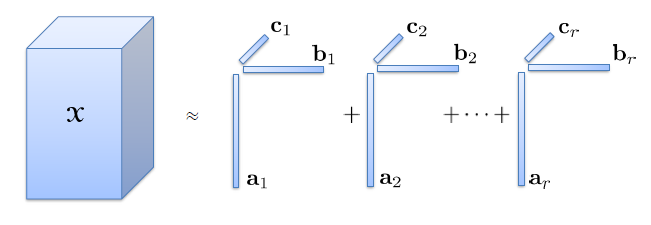
\includegraphics[width=0.4\linewidth,height=0.15\linewidth]{fig5.png}
	\caption{CP Decomposition}
	\label{fig5} 
\end{figure}
\begin{equation}
\mathop {\min }\limits_{A,B,C} {\left\| {\mathcal{X} - \mathcal{M}} \right\|^2}\;s.t.\;\;\mathcal{M} = \left[{A,B,C} 
\right] \Leftrightarrow \mathop {\min }\limits_{A,B,C} {\sum\limits_{i,j,k} {\left( {{x_{ijk}} - \sum\limits_l {{a_{il}}{b_{jl}}{c_{kl}}} } \right)} ^2}
\notag 
\end{equation}
unfortunately, it is nonconvex, but its subproblems are convex.

\vspace{0.25cm}

{\tiny There is a recommended Chapter 12 in Book {\color{blue} \cite{p4}}}.

\vspace{0.25cm}

{\tiny More details:} {\color{blue} \tiny \url{https://zhims.github.io/doc/note/datascience/LRS/tensor_2009.pdf}}. 

\end{frame}
%-----------------------------------------------------------------------------------------------

\begin{frame}
\frametitle{Tucker Decomposition}
\begin{figure}
	\centering
	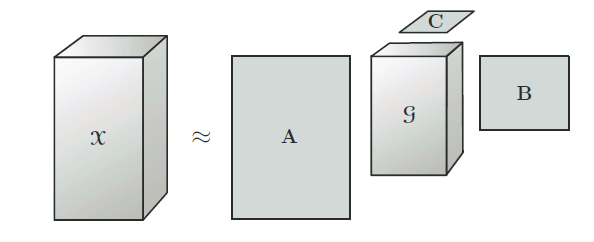
\includegraphics[width=0.4\linewidth,height=0.15\linewidth]{fig6.png}
	\caption{Tucker Decomposition}
	\label{fig6} 
\end{figure}
\begin{equation}
\mathop {\min }\limits_{\mathcal{G},A,B,C} {\left\| {\mathcal{X} - \mathcal{M}} \right\|^2}\;s.t.\;\;\mathcal{M} = \left[{\mathcal{G},A,B,C} 
\right]
\notag 
\end{equation}
\begin{center}
	where ${m_{ijk}} = \sum\limits_{{r_1}} {\sum\limits_{{r_2}} {\sum\limits_{{r_3}} {{g_{{r_1}{r_2}{r_3}}}{a_{i{r_1}}}} } {b_{j{r_2}}}{c_{k{r_3}}}} $
\end{center}

\vspace{0.25cm}

{\tiny There is a recommended Chapter 12 in Book {\color{blue} \cite{p4}}}.

\vspace{0.25cm}

{\tiny More details:} {\color{blue} \tiny \url{https://zhims.github.io/doc/note/datascience/LRS/tensor_2009.pdf}}.
\end{frame}
%-----------------------------------------------------------------------------------------------

\begin{frame}
\frametitle{\small Tensor-tensor Product}
\begin{definition}
	\small
	Let $ \mathcal{X} $ be an $ n_{1} \times {\color{red} n_{2}} \times {\color{blue} n_{3}} $ tensor and $ \mathcal{Y} $ be an $ {\color{red} n_{2}}  \times n_{4}\times {\color{blue} n_{3}} $ tensor. Then the t-product, denote by $ \mathcal{X}  * \mathcal{Y} $, is the $ n_{1} \times n_{4} \times n_{3} $ tensor given by
	
	\begin{equation}
	\mathcal{X} * \mathcal{Y} = fold(blockcirc (\mathcal{X}) \cdot unfold (\mathcal{Y}))
	\label{eq1}
	\end{equation}
	
	where {\tiny $blockcirc(\mathcal{X})  \doteq \left[ {\begin{matrix}
			{{X^{\left( 1 \right)}}} 		& {{X^{\left( n_3 \right)}}} 				&  \cdots  & {{X^{\left( 2 \right)}}}  \\ 
			{{X^{\left( 2 \right)}}} 		& {{X^{\left( 1 \right)}}} 				&  \cdots  & {{X^{\left( 3 \right)}}}  \\ 
			\vdots   		&  \vdots 				    			&  \ddots  &  \vdots  					 \\ 
			{{X^{\left( {{n_3}} \right)}}}  & {{X^{\left( {{n_3} - 1} \right)}}}    &  \cdots  & {{X^{\left( 1 \right)}}}  \\ 
			
			\end{matrix} } \right] \in {\mathbb{R}^{\left( {{n_1}{n_3}} \right) \times \left( {{n_2}{n_3}} \right)}}$, $unfold(\mathcal{Y})  \doteq \left[ {\begin{matrix}
			{{Y^{\left( 1 \right)}}}  \\ 
			{{Y^{\left( 2 \right)}}}  \\ 
			\vdots   \\ 
			{{Y^{\left( {{n_3}} \right)}}}  \\ 
			
			\end{matrix} } \right] \in {\mathbb{R}^{\left( {{n_2}{n_3}} \right) \times {n_4}}}$,}  \\
	
	\vspace{0.25cm}
	
	and the inverse operator fold takes $ unfold(\mathcal{X}) $ into a tensor: $ fold(unfold(\mathcal{Y})) = \mathcal{Y} $.
	\label{def1}
\end{definition}

\vspace{0.5cm}

{\tiny More details:} {\color{blue} \tiny \url{https://zhims.github.io/doc/note/datascience/LRS/tensor.pdf}}.

\end{frame}
%-----------------------------------------------------------------------------------------------

\begin{frame}
\frametitle{\small Tensor Decomposition based on tensor-tensor product via FFT}

\begin{theorem}[Tensor SVD]
	For any $ \mathcal{\mathcal{X}} \in \mathbb{R}^{n_{1} \times n_{2} \times n_{3}}$, the t-SVD of $ \mathcal{\mathcal{X}} $ is given by
	\begin{equation}
	\mathcal{\mathcal{X}} = \mathcal{U} * \mathcal{S} * \mathcal{V}^{T}
	\label{eq.1.17}
	\end{equation}
	where $ \mathcal{U} \in \mathbb{R}^{n_{1} \times n_{1} \times n_{3}} $ and $ \mathcal{V} \in \mathbb{R}^{n_{2} \times n_{2} \times n_{3}} $ are orthogonal, $ \mathcal{S} \in \mathbb{R}^{n_{1}\times n_{2} \times n_{3}} $ is f-diagonal.
\end{theorem}

\vspace{0.5cm}

{\tiny More details:} {\color{blue} \tiny \url{https://zhims.github.io/doc/note/datascience/LRS/tensor.pdf}}.

\end{frame}

%-----------------------------------------------------------------------------------------------

\begin{frame}
\frametitle{\small Tensor Decomposition based on Tensor-tensor Product via Unitary Transformation}

How about the topics in page {\color{blue} \ref{page12}} \& {\color{blue} \ref{page13}}?

\vspace{1cm}

How about the transformations, cosine, sine, wavelet, random matrix transformation? 

\end{frame}

%-----------------------------------------------------------------------------------------------

\section{Application \uppercase\expandafter{\romannumeral1}: Subspace Clustering}

%----------------------------------------------------------------------------------------------


\begin{frame}
\frametitle{ Section \uppercase\expandafter{\romannumeral4}}


\begin{center}
	\Large Application \uppercase\expandafter{\romannumeral1}: Subspace Clustering 
\end{center}

\end{frame}
%----------------------------------------------------------------------------------------------

\begin{frame}
\frametitle{ Subspace Clustering \uppercase\expandafter{\romannumeral1}}

\begin{equation}
\mathop {\min }\limits_Z {\lambda _1}{\left\| Z \right\|_*} + {\lambda _2}{\left\| Z \right\|_1} + \frac{{{\lambda _3}}}{2}\left\| {X - XZ} \right\|_F^2\;\;\;s.t.\;\;\;diag\;Z = 0,\;{1^T}Z = {1^T}
\end{equation}

In practice, ${\lambda _1} + {\lambda _2} = 1,\;$, choose $ \lambda_3 $ from paper {\color{blue}\cite{p3}}.

\vspace{0.5cm}

It is easy to show that the sequence generated by our algorithm is Cauchy sequence.

\vspace{0.5cm}

Now, how to choose $ \lambda_1, \lambda_2 $, and $ \lambda_3, \cdots $ by a simple MLP or CNN?

\end{frame}

%-----------------------------------------------

\begin{frame}
\frametitle{ \small Subspace Clustering \uppercase\expandafter{\romannumeral2}: Low-Rank Kernel Subspace Clustering}

Our model is 

\begin{equation}
\begin{split}
\mathop {\min }\limits_{C,D,F,E} \alpha \left\| C \right\|_{{l_{p_{1}}}}^{p_{1}}  + \beta \left\| C \right\|_{{S_{p_{2}}}}^{p_{2}} + \gamma \left\| {\Phi \left( Y \right) - \Phi \left( Y \right)C} \right\|_F^{\text{2}}
\end{split}
\end{equation}

How about 

\begin{equation}
\begin{split}
\mathop {\min }\limits_{B,C} & \left\| B \right\|_{_{{S_{{p_1}}}}}^{{p_1}} + {\lambda _1}\left\| B \right\|_{_{{l_{{p_2}}}}}^{{p_2}} + {\lambda _2}\left\| C \right\|_{{s_{{p_3}}}}^{{p_3}} + {\lambda _3}\left\| C \right\|_{{l_{{p_4}}}}^{{p_4}} \\
  + & \frac{{{\lambda _4}}}{2}\left\| {\phi \left( X \right) - \phi \left( X \right)C} \right\|_F^2 + \frac{{{\lambda _5}}}{2}\left\| {{K_G} - {B^T}B} \right\|_F^2
\end{split}
\label{eq13}
\end{equation}

\vspace{0.25cm}

{\tiny There is a recommended paper: {\color{blue} \url{https://arxiv.org/pdf/1707.04974v4.pdf}}}.

\vspace{0.25cm}


{\tiny And, more details:} {\color{blue} \tiny \url{https://zhims.github.io/doc/note/datascience/LRS/kernel.pdf}}.

\end{frame}

%-----------------------------------------------

\begin{frame}
\frametitle{ \small Subspace Clustering \uppercase\expandafter{\romannumeral2}: Low-Rank Kernel Subspace Clustering}

But there is a subproblem when we solve the Eq \ref{eq13}:
\begin{equation}
\small 
\mathop {\min }\limits_A \left\| {A + B} \right\|_F^2 + \left\| {{A^T}A + C} \right\|_F^2
\label{eq14}
\end{equation}

Problem \ref{eq14} can be written as
\begin{equation}
\small 
\mathop {\min }\limits_A Tr{\left( {A + B} \right)^T}\left( {A + B} \right) + Tr{\left( {{A^T}A + C} \right)^T}\left( {{A^T}A + C} \right)
\end{equation}
denote 
\begin{equation}
\small 
J = Tr{\left( {A + B} \right)^T}\left( {A + B} \right) + Tr{\left( {{A^T}A + C} \right)^T}\left( {{A^T}A + C} \right)
\end{equation}
then 
\begin{equation}
\small 
\frac{{\partial J}}{{\partial A}} = 2\left( {A + B} \right) + 4A{A^T}A + 4AC{C^T} = 0
\end{equation}
i.e.
\begin{equation}
\small 
A + 2A{A^T}A + 2AC{C^T} =  - B
\end{equation}

\end{frame}

%-----------------------------------------------

\begin{frame}
\frametitle{ Subspace Clustering \uppercase\expandafter{\romannumeral3 }}

\begin{equation}
\mathop {\min }\limits_{C,\mathcal{R}} \;\left\| {X - XC} \right\|_F^2 + \lambda \mathcal{R}\left( C \right)
\label{eq19}
\end{equation}

How to solve {\color{blue} \ref{eq19}}?

\vspace{0.25cm}

Deep proximal gradient.
\end{frame}

%-----------------------------------------------



\section{Application \uppercase\expandafter{\romannumeral2}: Salient Object Detection}

%----------------------------------------------------------------------------------------------
\begin{frame}
\frametitle{ Section \uppercase\expandafter{\romannumeral5}}


\begin{center}
	\Large Application \uppercase\expandafter{\romannumeral2}: Salient Object Detection
\end{center}

\end{frame}


%---------------------------------------------------------------------------------------------
\begin{frame}
\frametitle{Salient Object Detection}

\begin{equation}
\mathop {\min }\limits_{C,X,{\mathcal{R}}} \left\| {Y - XC} \right\|_F^2 + \mathcal{R}\left( C \right)
\end{equation}

or 

\begin{equation}
\mathop {\min }\limits_{f,\mathcal{R}} \left\| {Y - f\left( X \right)} \right\|_{F}^{2} + \lambda \mathcal{R}\left( X \right)
\end{equation}

or 

\begin{equation}
\begin{split}
\mathop {\min }\limits_{f,L.S,\mathcal{R}} \left\| {Y - f\left( X \right)} \right\| & + {\lambda _1}{\left\| L \right\|_*} + {\lambda _2}{\left\| S \right\|_1} + \left\langle {{Y_1},X - \left( {L + S} \right)} \right\rangle  \\
& + \frac{{{\lambda _3}}}{2}\left\| {X - \left( {L + S} \right)} \right\|_F^2 + \frac{{{\lambda _4}}}{2}\mathcal{R}\left( X \right)
\end{split}
\end{equation}



\end{frame}
%----------------------------------------------------------------------------------------------

\section{Application \uppercase\expandafter{\romannumeral3}: Linear Inverse Problems}

%----------------------------------------------------------------------------------------------
\begin{frame}
\frametitle{ Section \uppercase\expandafter{\romannumeral6}}


\begin{center}
	\Large Application \uppercase\expandafter{\romannumeral3}: Linear Inverse Problems
\end{center}

\end{frame}
%----------------------------------------------------------------------------------------------
\begin{frame}
\frametitle{Linear Inverse Problems \uppercase\expandafter{\romannumeral1}}

It is a typical ill-posed linear inverse problem and can be generally formulated as:

\begin{equation}
\boldsymbol{y} = H \boldsymbol{x} + \boldsymbol{n}
\label{eq1.1}
\end{equation}

where $ \boldsymbol{x}, \boldsymbol{y} $ are lexicographically stacked representations  of the original image and the degraded image, respectively, $ H $ is a matrix representing a non-invertible linear degradation operator and $ \boldsymbol{n} $ is usually additive Gaussian white noise. 


Our model:

\vspace{-0.15cm}

\begin{equation}
\mathop {\arg \min }\limits_{{{\bf{x}}_i}} \:\frac{1}{2}\sum\limits_{i = 1}^3 {\left\| {H{x_i} - {y_i}} \right\|_2^2}  + \lambda {\left\| {\left( {ten\left[ {mat\left( {{x_1}} \right),mat\left( {{x_2}} \right),mat\left( {{x_3}} \right)} \right]} \right)} \right\|_*}
\end{equation}

{\tiny More details:} {\color{blue} \tiny \url{https://zhims.github.io/doc/note/datascience/LRS/GSR.pdf}}.
\end{frame}

%----------------------------------------------------------------------------------------------
\begin{frame}
\frametitle{Linear Inverse Problems \uppercase\expandafter{\romannumeral2}}

{\tiny There is a recommended slides {\color{blue} \url{https://imaging-in-paris.github.io/semester2019/slides/w1/willett.pdf}}}.

\vspace{0.5cm}

{\tiny And, there are two  recommended papers: 
	
	\vspace{0.25cm}
	
	\begin{enumerate}
		\item IEEE Transactions on Computational Imaging:  {\color{blue} \url{https://arxiv.org/pdf/1901.03707.pdf}}.
		
		\vspace{0.5cm}
		
		\item IEEE Journal on Selected Areas in Information Theory: {\color{blue} \url{https://arxiv.org/pdf/2005.06001.pdf}}.
	\end{enumerate}
}

\vspace{0.5cm}

{\tiny More details:} {\color{blue} \tiny \url{https://zhims.github.io/doc/note/datascience/LRS/NeumannNetworks.pdf}}.


\end{frame}
%----------------------------------------------------------------------------------------------


\section{References}
%------------------------------------------------
\begin{frame}
\frametitle{References}
\footnotesize{
	\begin{thebibliography}{99} % Beamer does not support BibTeX so references must be inserted manually as below
		\bibitem[Udell et al, 2018]{p1} M. Udell  and A. Townsend (2018)
		\newblock Why Are Big Data Matrices Approximately Low Rank?
		\newblock \emph{SIAM Journal on Mathematics of Data Science}, Vol1(1):144-160, 2018.
	\end{thebibliography}
	\begin{thebibliography}{99} 
		\bibitem[Scetbon et.al  2020]{p2}M. Scetbon, M. Elad and P. Milanfar(2020)
		\newblock Deep K-SVD Denoising
		\newblock \emph{IEEE Selected Topics in Signal Processing (Special Issue on Deep Learning for Image/Video Restoration and Compression)}
	\end{thebibliography}
	\begin{thebibliography}{99} 
		\bibitem[Elhamifar et al, 2013]{p3} E. Elhamifar and R. Vidal (2013)
		\newblock Sparse Subspace Clustering: Algorithm, Theory, and Applications
		\newblock \emph{IEEE Transactions on Pattern Analysis and Machine Intelligence}, Vol35(11):2765--2781, 2013.
	\end{thebibliography}
	\begin{thebibliography}{99} 
		\bibitem[Golub et al, 2013]{p4} G. Golub and C. Van Loan (2013)
		\newblock Matrix Computations
		\newblock \emph{Johns Hopkins University Press}, 2013.
	\end{thebibliography}
	\begin{thebibliography}{99}
		\bibitem[Kolda et al, 2009]{p5} T. Kolda and B. Bader (2009)
		\newblock  Tensor Decompositions and Applications
		\newblock \emph{SIAM Review}, Vol51(3): 455-500, 2009.
	\end{thebibliography}
}
\end{frame}
%-------------------------------------------------------------------------------------------

%-------------------------------------------------------------------------------------------

\begin{frame}
\frametitle{Highly Recommended Book}
\begin{center}
	\color{magenta}
	
	High-Dimensional Data Analysis with Low-Dimensional Models: 
	
	\vspace{0.25cm}
	
	Principles, Computation, and Applications
	
	\vspace{0.55cm}
	
	Authors: John Wright and Yi Ma
	
	\vspace{0.5cm}
	
	{\color{blue}\tiny \url{https://book-wright-ma.github.io/Book-WM-20201206.pdf}}{\color{black}.}
\end{center}
\end{frame}
%----------------------------------------------------------------------------------------


%----------------------------------------------------------------------------------------



%-------------------------------------------------------------------------------------------
\begin{frame}
\frametitle{The End}
\begin{center}
	{\Huge Thank you!}
	
	\vspace{1cm}
	
	{\Huge Any comments or questions?}
	
	\vspace{2.25cm}	
	
  {\tiny Welcome to visit my personal homepage: \ {\color{blue} \url{https://zhims.github.io/}}}
\end{center}
\end{frame}
%----------------------------------------------------------------------------------------
%----------------------------------------------------------------------------------------

\end{document} 